\subsection{Skew halda} 
Skew halda je jednou zo samoupravujúcich sa háld. To znamená, že negarantuje dobrú časovú zložitosť pre najhorší prípad, ale stará 
sa o to, aby v budúcnosti robila operácie efektívnejšie. Pri takomto druhu haldy sa pozeráme na \emph{amortizovanú časovú 
zložitosť}. Nezaujíma nás časová zložitosť pre najhorší prípad, ale priemerná zložitosť postupnosti operácií.

\paragraph{Popis.}
Skew halda je odvodená z ľavicovej haldy. Jediný rozdiel je, že pre skew haldu nedefinujeme rank. Teda je to opäť druh binárnej 
haldy. Taktiež jej hlavnou výhodou je spájanie, je však jednoduchšia na implementáciu.


\paragraph{Operácie.}
Prvá fáza operácie \emph{meld(i,j)} na skew halde je totožná s ľavicovou haldou. Keďže ranky tu neexistujú, druhá fáza spájania 
ľavicových háld sa preskočí a prejdeme k poslednej fáze. Táto časť obsahuje kľúčovú úpravu haldy, ktorá zabezpečuje efektívne 
spájanie. Postupujeme po pravej spájacej ceste haldy, ktorá vznikla v prvom kroku. Začneme v predposlednom vrchole%
\footnote{Keďže posledný vrchol nemá pravého syna, nemá zmysel mu vymieňať synov, nanajvýš by sme tým predĺžili pravú cestu.} 
smerom nahor až po koreň. Každému vrcholu po ceste vymeníme synov.


\begin{figure}
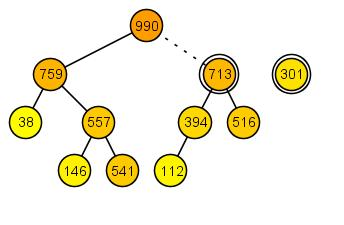
\includegraphics[width=\columnwidth]{obrazky/skewinsert.png}
\caption{\emph{Spájanie pozdĺž pravej cesty.}} 
\label{img:skew} 
\end{figure}

Zvyšné operácie sú definované rovnako, ako pri ľavicovej halde.

\paragraph{Časová zložitosť.}
Amortizovaná časová zlotosť pre $\meld(i,j)$ je $O(\log n)$.
Takisto platí aj pre $\ins(x)$, \emph{deleteMin} a $\dec(v,\Delta)$ \citep{skew}.
Ku skew halde tiež existujú alternatívy -- top-down, bottom-up. 
Bottom-up prístup ohraničuje všetky operácie až na \emph{deleteMin} na $O(1)$.
\emph{DeleteMin} má v tomto prípade časovú zložitosť $O(\log n)$.
